\scanpage{11}
\deleted{\uline{\unsure{Exemple|Corollaire}}}

\uline{Remarques} 1) La condition (i) est peut être néc. et \unsure{suffisante|suffisant|suffit} pour l'existence d'un \uline{$M$} \uline{non néc. séparé} sur $Y$.

2) La condition (i) \inserted{\deleted{et (iii)}} est satisfaite si $f$ est un morphisme \uline{séparable}. Si $f$ est de plus propre, alors \inserted{(iii) est satisfait. De plus,} le nb $\unsure{\nu|v}(y)$ des composantes irréductibles relatives (non néc. déf $/\,k(y)$) est tj continue supérieurement, \inserted{Alors} \deleted{la condition} \deleted{La conjonction de (ii) et (iii) \unsure{(iii)}, est nécessairement satisfaite,} \deleted{(ii) \unsure{équiv}} équivalence entre les conditions suivantes

a) Condition (ii) plus haut de non \unsure{scindage} d'une composante ult\textsuperscript{t} irréd. par spécialisation

b) $\nu$ est \unsure{loc|donc} constante

c) $M$ existe

\deleted{Et} Alors $M$ est \uline{propre} sur $Y$.

\figure{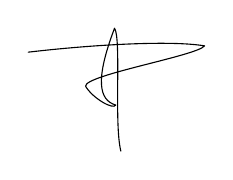
\begin{tikzpicture}[x=.8cm,y=.8cm,line join=round,line cap=round]
 \draw (.0,1.57) .. controls (1.03,1.69) and (2.26,1.76) .. (2.80,1.67)
 .. controls (2.67,1.51) and (.90,1.21) .. (.91,1.03)
 .. controls (1.02,.84) and (1.35,.65) .. (1.39,.73)
 .. controls (1.12,.81) and (1.06,1.13) .. (1.37,1.95)
 .. controls (1.48,1.79) and (1.36,.44) .. (1.47,0);
\end{tikzpicture}}
% archive sheet number: 10
